\documentclass[letterpaper]{article}  

\usepackage{graphicx}
\usepackage{float}
\usepackage[margin=0.5in]{geometry}
\usepackage{caption}
\usepackage{subcaption}

\usepackage{Sweave}
\begin{document}
\Sconcordance{concordance:HW1-sweave.tex:HW1-sweave.Rnw:%
1 8 1 1 0 157 1}


\title{STA511 Homework \#1}
\date{September 30, 2015}
\author{Abbas Rizvi}
\maketitle

\begin{enumerate}

\item No work required for question 1

\item My answer to \# 2, has multiple parts.

\begin{enumerate}
\item X is distributed as a uniform random variable $X$ $\sim$ $U(0,1))$ and was simulated 1000 times (Figure 1 - Left panel). A second histogram was generated plugging in $X$ into the formula $Y = $ $\pi$$X - \frac{\pi}{4}$ (Figure 1 - Right panel).
\begin{figure}[htpb]
\centering
\caption{Histograms of $(X$ $\sim$ $U(0,1))$ (Left panel) and $Y = $ $\pi$$X - \frac{\pi}{4}$ (Right panel) simulated 1000 times}
\centering

\includegraphics[scale=0.6]{/Users/aarizvi/Desktop/ROSWELL_PHD/STA511_StatisticalComputing/HW1/hw1-q2a-runiform-histogram.pdf}
\end{figure}
\\
The R code used for question 2 part a was:
\begin{verbatim}
#part 2a-1
runif.histogram <- runif(1000,0,1)

#part 2a-2
x <- runif.histogram
y <- 3.14*x + 3.14/4

pdf("hw1-q2a-runiform-histogram.pdf")
par(mfrow=c(1,2),bg="gray")
hist(runif.histogram, main="X ~ U(0,1) Simulations", xlab = 'X', breaks=25)
hist(y, main="Y = pi/X - (pi/4) Simulations", xlab = 'Y = pi/X - (pi/4), breaks=20)
dev.off()
\end{verbatim}

\item Looking at the histogram in Y (Figure 1 - Right panel), the distribution appears to be uniform. My guess for the theoretical distribution is $f(x) = \frac{1}{B - A}$ for $A \leq X \leq B$. 

\item 1000 random samples were generated for $Z$, another uniform random variable ($Z$ $\sim$ $U(0,1))$ The samples were generated using two separate R functions {\tt{hist()}} and {\tt{truehist()}} and subsequently compared.
\\
The R code used to generate question 2 part c was:
\begin{verbatim}
#2c 
z <- runif(1000,0,1)
xpz <- x + z
pdf("hw1-q2c-xpz.pdf")
hist(xpz,breaks=15,col="green",main="hist(X + Z)")
dev.off()

#2d
library(MASS)
pdf("hw1q2d-truehist.pdf")
truehist(xpz,main="truehist(X + Z)",ylab="probability")
dev.off()
\end{verbatim}

\begin{figure}
    \centering
    \caption{1000 random samples were generated for $Z$, another uniform random variable ($Z$ $\sim$ $U(0,1))$ using {\tt{hist()}} and {\tt{truehist()}}.}
    \begin{subfigure}{0.4\textwidth}
        \centering
        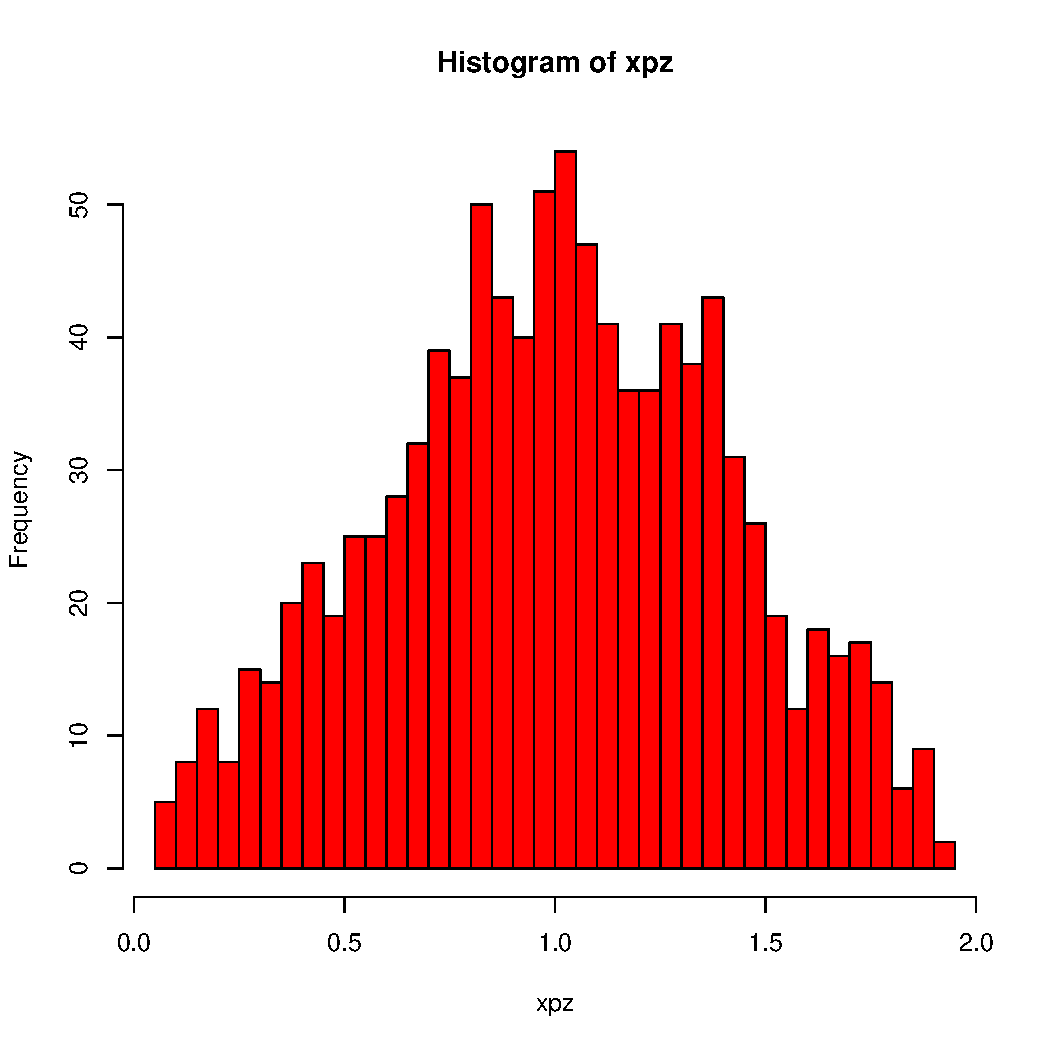
\includegraphics[width=\textwidth]{/Users/aarizvi/Desktop/ROSWELL_PHD/STA511_StatisticalComputing/HW1/hw1-q2c-xpz.pdf}
        \caption{{\tt{hist(X + Z)}}}
    \end{subfigure}
    \begin{subfigure}{0.4\textwidth}
        \centering
        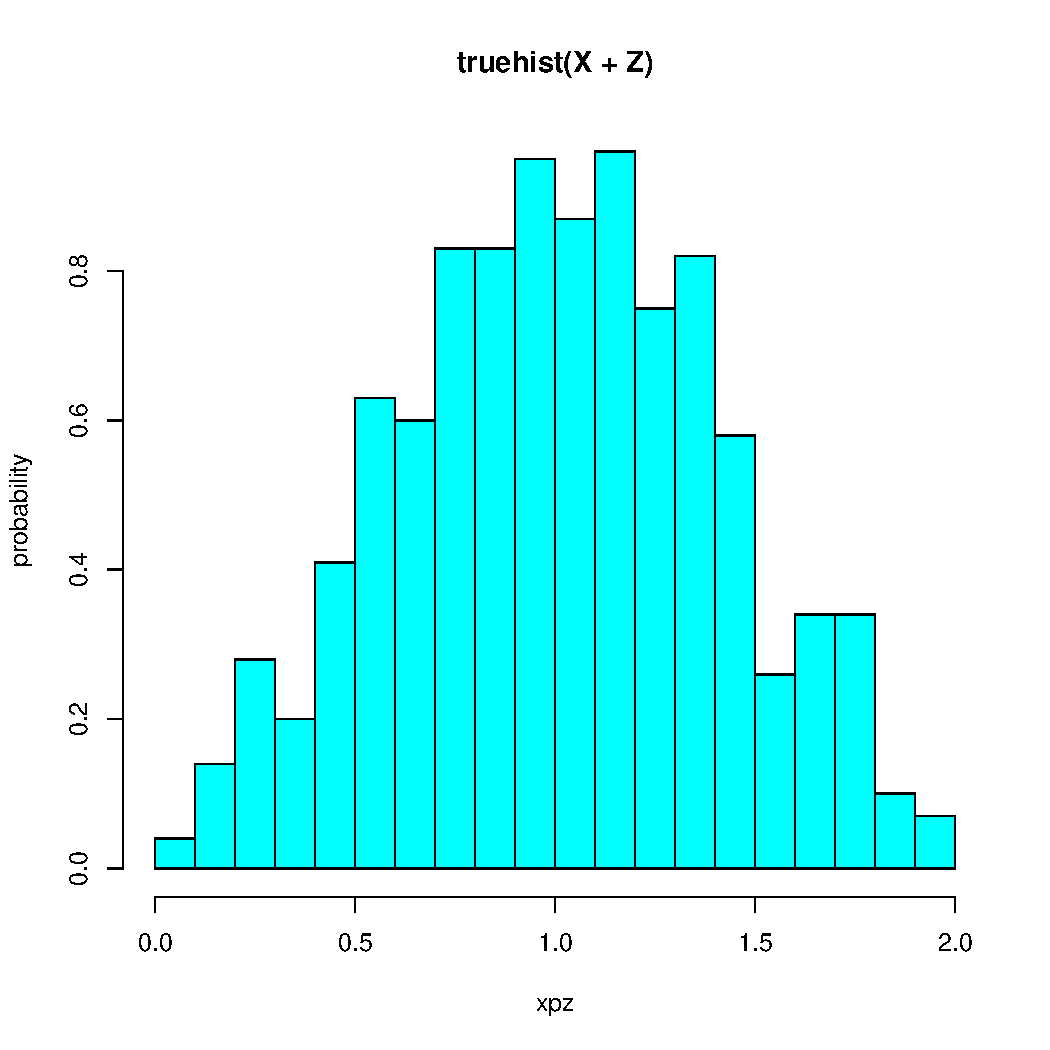
\includegraphics[width=\textwidth]{/Users/aarizvi/Desktop/ROSWELL_PHD/STA511_StatisticalComputing/HW1/hw1q2d-truehist.pdf} 
        \caption{{\tt{truehist(X + Z)}}}
    \end{subfigure}
\end{figure}

\item{The y-axis in {\tt{hist()}} is relative frequency (Figure 2a) and the y-axis from {\tt{truehist()}} is the probability (Figure 2b).}

\item{The histograms look like they are normally distributed, so the distribution is approximately: \\
$f(x \; | \; \mu, \sigma) = \frac{1}{\sigma\sqrt{2\pi} } \; e^{ -\frac{(x-\mu)^2}{2\sigma^2}}$}

\end{enumerate} 

\item Thirty grade randomly uniform observations were generated from 60 and 100 and attached to the STA 511 course roster (Table 1). The corresponding letter grade was attached to the column next to the right of the randomly generated observations (Table 1).  

\begin{table}[ht]
\caption{STA 511 Course Roster Randomized Grades and Corresponding Letter Grade}
\centering
\begin{tabular}{rlllrl}
  \hline
 & Name & Program.and.Plan & Level & Percent.Grade & Letter.Grade \\ 
  \hline
1 & An,Bo & Pharmaceutcl Sci Doctoral  & Doctoral 2 & 73.00 & C \\ 
  2 & Bu,Yahao & Public Health Masters  & Masters 2 & 68.54 & C \\ 
  3 & Chang,Huiru & Public Health Masters  & Masters 2 & 63.61 & C \\ 
  4 & Chen,Jiangwang & Public Health Masters  & Masters 2 & 71.97 & C \\ 
  5 & Eum,Youngseob & Arts \& Sciences Doctoral  & Doctoral 1 & 74.52 & C \\ 
  6 & Ganley,Kevin & Public Health Masters  & Masters 1 & 67.26 & C \\ 
  7 & Hess,Katelyn & Arts \& Sciences Masters  & Masters 1 & 84.34 & B \\ 
  8 & Hsu,En-Shuo & Public Health Masters  & Masters 1 & 80.25 & B \\ 
  9 & Jai Kumar Ahuja,Suruchi & Public Health Masters  & Masters 1 & 82.86 & B \\ 
  10 & Jin,Yuxuan & Public Health Doctoral  & Doctoral 1 & 79.65 & B- \\ 
  11 & Karaesmen,Ezgi & Roswell Park Doctoral  & Doctoral 2 & 76.51 & B- \\ 
  12 & Krishnan,Krithika & Public Health Masters  & Masters 1 & 89.05 & B+ \\ 
  13 & Lin,Jieya & Public Health Masters  & Masters 1 & 95.36 & A \\ 
  14 & Mandava,Aishwarya & Public Health Masters  & Masters 1 & 99.15 & A \\ 
  15 & Marsales,Harry & Public Health Masters  & Masters 2 & 68.66 & C \\ 
  16 & Morrell,Kayla & Public Health Masters  & Masters 1 & 83.43 & B \\ 
  17 & Niu,Jin & Pharmaceutcl Sci Doctoral  & Doctoral 2 & 91.37 & A- \\ 
  18 & Rizvi,Abbas & Roswell Park Doctoral  & Doctoral 2 & 92.22 & A- \\ 
  19 & Rosario,Spencer Rae & Roswell Park Doctoral  & Doctoral 2 & 84.09 & B \\ 
  20 & Schiller,Emily & Public Health Masters  & Masters 1 & 99.41 & A \\ 
  21 & Song,Jiaming & Public Health Masters  & Masters 1 & 87.51 & B+ \\ 
  22 & Spencer,Mary & Public Health Masters  & Masters 1 & 65.71 & C \\ 
  23 & Sun,Xiaoxi & Public Health Masters  & Masters 1 & 97.25 & A \\ 
  24 & Tanue,Terence Wankah & Public Health Masters  & Masters 1 & 69.08 & C \\ 
  25 & Tian,Mingmei & Public Health Masters  & Masters 2 & 63.18 & C \\ 
  26 & Vucic,Luther & Public Health Masters  & Masters 1 & 78.60 & B- \\ 
  27 & Wackeroth,Wolf Michael & Public Health Masters  & Masters 1 & 68.49 & C \\ 
  28 & Wang,Jiefei & Public Health Masters  & Masters 1 & 93.77 & A- \\ 
  29 & Wang,Xue & Roswell Park Doctoral  & Doctoral 2 & 89.14 & B+ \\ 
  30 & Wu,Yin & Grad Sch of Ed Doctoral  & Doctoral 2 & 86.43 & B+ \\ 
  31 & Yang,Yang & Grad Sch of Ed Doctoral  & Doctoral 2 & 85.94 & B+ \\ 
  32 & Yang,Yujie & Pharmaceutcl Sci Doctoral  & Doctoral 2 & 81.69 & B \\ 
  33 & Yang,Zeyu & Public Health Masters  & Masters 1 & 63.28 & C \\ 
  34 & Yu,Xinyang & Biomedical Sci Doctoral  & Doctoral 2 & 78.93 & B- \\ 
  35 & Zhao,Yichen & Grad Sch of Ed Doctoral  & Doctoral 2 & 62.93 & C \\ 
   \hline
\end{tabular}
\end{table}

Here is my code:
\begin{verbatim}
#question 3
class.roster <- read.table("classlist.txt",sep="\t",header=TRUE)
Percent.Grade <- runif(35, 60, 100)
class.roster.2 <- cbind(class.roster, Percent.Grade)
class.roster.2 <- data.table(class.roster.2)

#remove weird -\xa0 symbol
class.roster.2$Program.and.Plan <- gsub("[-\xa0]", "",class.roster.2$Program.and.Plan)

library(data.table)
class.roster.2[Percent.Grade > 95, Letter.Grade := "A"]
class.roster.2[Percent.Grade >= 90 & Percent.Grade < 95, Letter.Grade := "A-"]
class.roster.2[Percent.Grade >= 85 & Percent.Grade < 90, Letter.Grade := "B+"]
class.roster.2[Percent.Grade >= 80 & Percent.Grade < 85, Letter.Grade := "B"]
class.roster.2[Percent.Grade >= 75 & Percent.Grade < 80, Letter.Grade := "B-"]
class.roster.2[Percent.Grade < 75, Letter.Grade := "C"]

install.packages('xtable')
library(xtable)

roster.table <- xtable(class.roster.2)
print(roster.table)

\end{verbatim}

\end{enumerate}
\end{document}
